\label{sec:Res}
\section*{Results}

We partitioned variance due to the species effect, i.e. the part of the variance explained by the species of individuals (see~\autoref{fig:aov}). Depending on the trait, the species effect could explain between 27\% up to 75\% of the variability of our data. While species effect can explain over 75\% of the variability in wood density, it only explains less than 30\% of the variability in AGR.

%Several other factors may explain residual variability: micro-environmental conditions, intra-specific variability or climatic conditions for example. In order to disentangle better the residual variance, we tested spatial auto-correlation of traits and AGR on our plots with mark correlation functions (data not shown). Neither traits nor AGR were spatially auto-correlated, i.e. the distribution of AGR or trait values in our 9 plots is not specifically distributed, indeed it is not very different from random distribution of those values in the plots. It underlines that in our data set the micro-environment does not strongly influence the traits.

To test how growth was affected by individual traits we made growth mixed-model for each one of them (see~\autoref{tab:seltraits} for traits and~\autoref{tab:growth_mod} for models) as predictors of the AGR. All the models included a plot and a species random effects, as well as fixed DBH and $\log(\text{DBH})$ terms. For each trait, with the aforementioned effects plus one term that included as a fixed effect: the species average trait, the species average trait plus a distance term (hierarchical or absolute) to individual's trait, or the individual's trait value. Based on the adapted R-squared for mixed-models~\citep{nakagawa_general_2013}, we then selected the best model for each trait (see~\autoref{tab:growth_mod}).

For all traits models with distance measures were better than model with only species average term. But for wood density and SLA, hierarchical distances model performed as well as indvidual's trait models. By adding a distance term to the species average term model, we gained in predictive power, shown by the increase of condition R-squared between models. For bark thickness the absolute distance model improved the conditional R-squared by 0.025 compare to the model with only species average trait; for wood density hierarchical distance model improved the R-squared by 0.056 (10\% of total $\text{R}^2$) compared to species average model; for SLA hierarchical distance model only increased $\text{R}^2$ by 0.004; For laminar chlorophyll and toughness the same model gained 0.001 of R-squared compared to the species average term models.

Using the best models (in bold in~\autoref{tab:growth_mod}) that included a distance term we predicted AGR for a range of individual trait values and species average values. To underline the interplay between intra- and inter-specific variabilities we plotted the centered species average trait value vs. the hierarchical distance of indivdual's (see~\autoref{fig:simul}). We obtained AGR "landscapes", that show the pattern of variations of variation as a function of individual and species trait variation. Depending on the trait we had different patterns, for SLA and wood density we had similar patterns: the larger the species average trait value, the lower the AGR, and the higher the individual's hierarchical distance the lower the AGR. For example, an increase of $3\text{cm}^2.\text{g}^{-1}$ from the centered species average decreases the growth by $0.005\text{mm}.\text{yr}^{-1}$ while the same increase in hierarchical distance decreases the AGR by $0.01\text{mm}.\text{yr}^{-1}$. For laminar chlorophyll content we observe that increasing centered species average as well as increasing hierarchical distance lead to increasing AGR. While for leaf toughness, centered species average and hierarchical AGR gradients are opposed: an increase in centered species average decreases AGR, and an increase individual's hierarchical distance increases AGR. Because the best model for bark thickness was an absolute distance model, we observe the symmetrical patterns of AGR variations for change in hierarchical distance: globally, the higher the hierarchical distance the lower the AGR, while the higher the species average, the lower the growth.

\begin{table}[!t]
	\begin{center}
		\begin{tabular}{llcccc}
		  \hline
		 Trait Name & Model Type & Marginal $\text{R}^2$ & Cond. $\text{R}^2$ & AIC & logLikelihood \\ 
		  \hline
		Bark Thickness & Species Avg. & 0.104 & 0.472 & -2790 & 1407 \\ 
		            & Hierarchical Distance & 0.106 & 0.471 & -2794 & 1410 \\ 
		            & \textbf{Absolute Distance} & 0.100 & \textbf{0.497} & -2860 & \textbf{1443} \\ 
		            & Individual Trait & 0.102 & 0.470 & -2792 & 1408 \\
		  \cline{2-6}
		  Wood Density & Species Avg. & 0.142 & 0.474 & -1838 & 931 \\ 
		               & \textbf{Hierarchical Distance} & 0.139 & \textbf{0.530} & -1910 & \textbf{968} \\ 
		               & Absolute Distance & 0.140 & 0.529 & -1906 & 966 \\ 
		               & \textbf{Individual Trait} & 0.137 & \textbf{0.530} & -1911 & \textbf{968} \\
		  \cline{2-6}
		  SLA & Species Avg. & 0.094 & 0.485 & -3081 & 1553 \\ 
		      & \textbf{Hierarchical Distance} & 0.095 & \textbf{0.489} & -3092 & \textbf{1559} \\ 
		      & Absolute Distance & 0.096 & 0.459 & -3000 & 1513 \\ 
		      & \textbf{Individual Trait} & 0.096 & \textbf{0.490} & -3093 & \textbf{1559} \\ 
		  \cline{2-6}
		  Chloro. Content & Species Avg. & 0.092 & 0.487 & -3143 & 1583 \\ 
		                  & \textbf{Hierarchical Distance} & 0.093 & \textbf{0.488} & -3145 & \textbf{1586} \\ 
		                  & Absolute Distance & 0.092 & 0.486 & -3143 & 1584 \\ 
		                  & Individual Trait & 0.100 & 0.469 & -3075 & 1550 \\
		  \cline{2-6}	
		  Toughness & Species Avg. & 0.088 & 0.478 & -3136 & 1580 \\ 
		            & \textbf{Hierarchical Distance} & 0.088 & \textbf{0.479} & -3135 & \textbf{1581} \\ 
		            & Absolute Distance & 0.088 & 0.478 & -3134 & 1580 \\ 
		            & Individual Trait & 0.088 & 0.479 & -3134 & 1579 \\
		   \hline
		\end{tabular}
		\caption{\textbf{Summary table of tested trait-specific growth models.} We modeled radial growth using linear-mixed model, all models contained plot and species random effects, as well as DBH and $\log\text{DBH}$ terms to take growth curve shape into account~\citep{herault_functional_2011}. Then, for each trait, we added a fixed effect that contained different terms: \textbf{Species Avg.}, only the species average trait value; \textbf{Hierarchical Distance}, the species average plus the difference between individual's trait and species average; \textbf{Absolute Distance}, the species average plus the absolute difference between individual's trait and species average; \textbf{Individual Trait}, only the trait value of individuals. Models indicated in \textbf{bold} are those with the highest logarithmic likelihood per trait.}
		\label{tab:growth_mod}
	\end{center}
\end{table}

\begin{figure}[!tb]
	\centering
	\begin{subfigure}[c]{0.45\textwidth}
		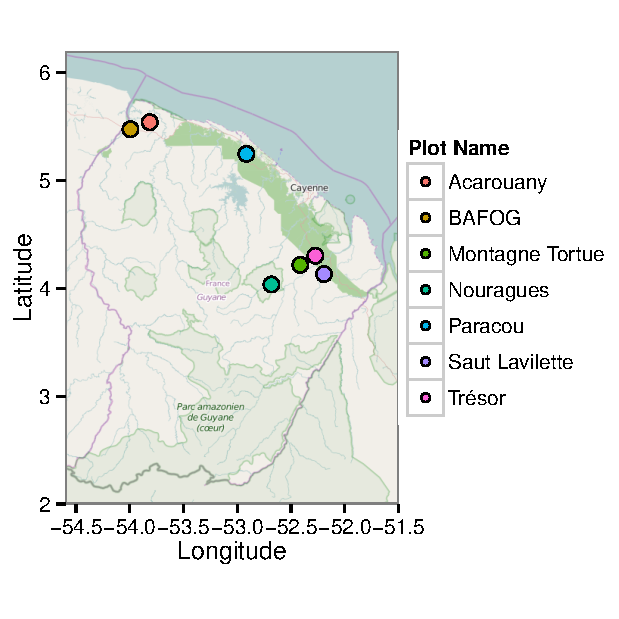
\includegraphics[scale=0.75]{figures/Plots_Map_2015-05-26.pdf}
		\caption{}
		\label{fig:map}
	\end{subfigure}
	\begin{subfigure}[c]{0.5\textwidth}
		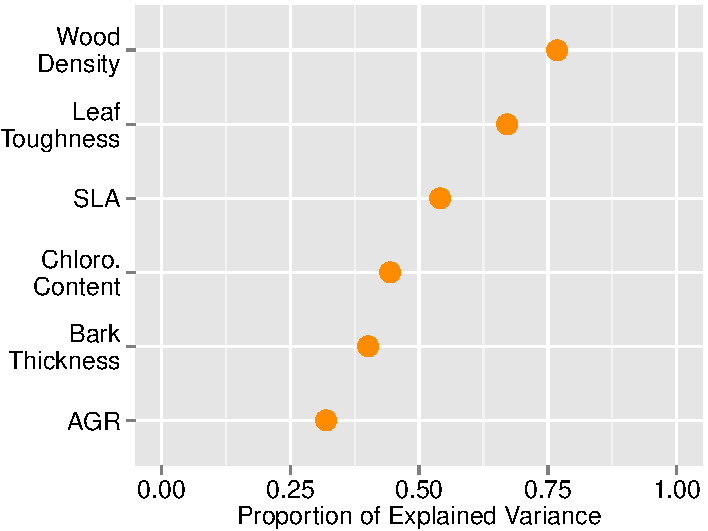
\includegraphics[scale=0.7]{figures/Aov_Var_Traits_2015-05-25.pdf}
		\caption{}
		\label{fig:aov}
	\end{subfigure}
	\caption{\textbf{(a) Plots map.} 9 1-ha plots were used, spread in French Guiana, two plots were surveyed both in Nouragues and in Paracou (see~\citealp{baraloto_decoupled_2010}) \textbf{(b) Explained variance by species effect in ANOVAs.} Dot-plot of explained variance in ANOVA by the species effect for traits and AGR. \textbf{Chloro. Content}: Laminar Chlorophyll Content, \textbf{AGR}: Annual Growth Rate (in diameter).}
	\label{fig:gen}
\end{figure}

\begin{figure}[!tb]
	\centering
	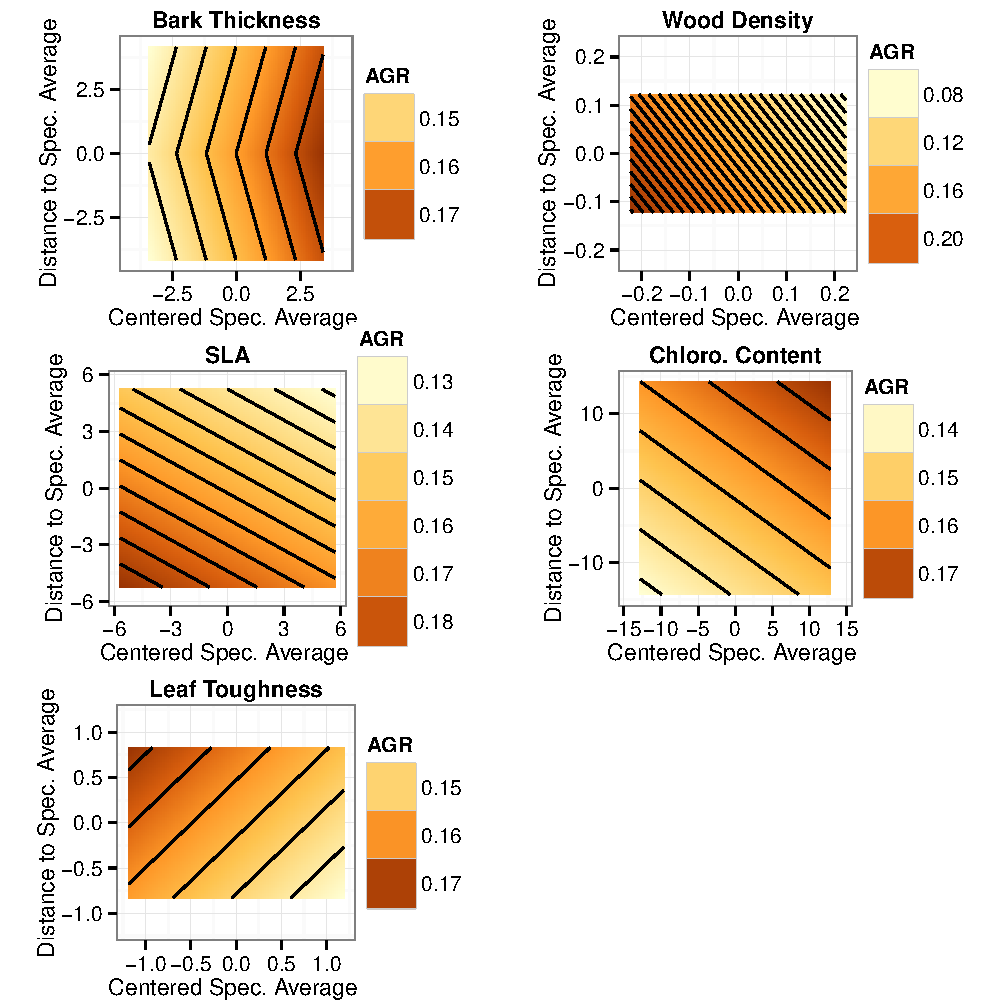
\includegraphics{figures/Sel_Traits_Simul_AGR_2015-05-28.pdf}
	\caption{\textbf{Simulations of species trait and predictions of AGR with growth models.} Surface plots of predicted AGR of simulated range of data: X-axis, centered species average trait (species average trait minus mean of all species average trait); Y-axis, individual distance to species average trait. Black lines are equal-AGR lines over the surface, i.e. on those line each point has the same AGR value, each line mark a $5e^{-3}\text{mm}.\text{yr}^{-1}$ break. For details on traits see~\autoref{tab:seltraits}.}
	\label{fig:simul}
\end{figure}